\section{Embedded RT Systems}
\subsection{Definition Embedded Systems}
Embedded computer system: A computer system that is part of a larger system and performs some of the requirements of that system.
For example, a computer systesm used in an aircraft of rapid transit system.\\
An embedded system consists of four main components:
\begin{itemize}
  \item Processor (microprocessor or microcontroller)
  \item Memory (RAM and ROM)
  \item Peripherals (input and output)
  \item Software (main programm)
\end{itemize}

\subsection{Definition Real-time}
\begin{description}
  \item[Defininition:] A real-time system is a computing system whose correct behavior depends not only on the \textbf{value of the computation} but also on the \textbf{time} at which outputs are produced.
  \item[Determinism:] A system behaves always the same time and same way.
        There is no randomness.
  \item[Hard Time Constraint:] The consequence of a missed deadline is fatal.
        A late response is useless, and sometimes totaly unacceptable.
  \item [Soft Time Constraint:] Consequence of a missed deadline is undesirable but tolerable.
        A late response is still useful as long as it is within some acceptable range.
  \item [Hard real-time system:] A real-time system is capable to solve all real-time specific tasks, under all circumstances, within a defined time span.
  \item [Soft real-time system:] A soft real-time system is capable to solve a specific task, under most circumstances, within a defined time span.
\end{description}

\subsubsection{Application}
The application defines \ldots
\begin{itemize}[label=\ldots]
  \item the deadlines and may have a bandwidth
  \item what occurs if a deadline is missed (overheating, vehicle gets out of control)
  \item what are the consequences when a deadline is missed (comfort loss, unsatisfied customer, crash)

\end{itemize}
Design defines how to meet the requirements:
\begin{itemize}
  \item Hardware architecture (CPU platform)
  \item Software architecture (programming language an elements, no OS, Interrupt concept, OS)
\end{itemize}
\textbf{Requirements} and \textbf{system design} are \textbf{key} to \textbf{solve real time} applications.

\subsection{Goal / Benchmarks of an embedded Real Time System}
An embedded real time system can be evaluated in three aspects:
\begin{description}
  \item [Service:] How reliable are the flows and the results done.
  \item [Deterministic:] How well are the deadlines met.
  \item [Energy:] How much energy is needed to solve the application.
        Idle state needs energy whiteout sleep modes.
\end{description}

\subsection{Special Requirements}
\begin{itemize}
  \item Reactive functionality
        \begin{itemize}
          \item An embedded-system has to react on external events
          \item Many events can happen at the same time
        \end{itemize}
  \item Hard Real-time requirements
        \begin{itemize}
          \item Has to react within a defined time
          \item Otherwise it is unusable or it can even cause harm
        \end{itemize}
  \item Reliability
        \begin{itemize}
          \item May be safety critical
          \item Softwaren-updates expensive
          \item Faults can cause material damage
        \end{itemize}
  \item Economic efficiency
        \begin{itemize}
          \item High number of units
          \item Power consumption
          \item Battery size
          \item Unit cost
        \end{itemize}
  \item Extreme environmental conditions
        \begin{itemize}
          \item Electromagnetic Compatibility (EMC), temperature, …
        \end{itemize}
  \item Product lines
  \item Testability
\end{itemize}


\subsection{Technology Overview}
The hardware is like a foundation of the system.
It lays the first layer of constraints for real time operation.
\begin{itemize}
  \item How many cycle needs the memory load and store mechanism?
  \item Are there commands that last longer than one instruction cycle?
  \item Can a command with more than one instruction cycle be interrupted?
  \item How much time is needed to interrupt a interrupt process?
  \item Can an interrupt be interrupted (interrupt nesting)?
\end{itemize}

\subsubsection{Types of Microcontrollers / Microprocessors}
\begin{tabularx}{\textwidth}{l X X X}\hline
          & Single Microcontroller & Symmetrical Multicore \textmu{}P/\textmu{}C & Asymmetrical Multicore \textmu{}P/\textmu{}C \\\hline
  Example & STM32F429 (Cortex M4)  & ARM Cortex A72 (A72)                        & STM32H7x5/7X7 \linebreak(Cortex M4/M7)       \\
  Board   & 32F429IDISCOVERY       & Raspberry Pi 4                              & NUCLEO-H745ZI-Q                              \\\hline
\end{tabularx}

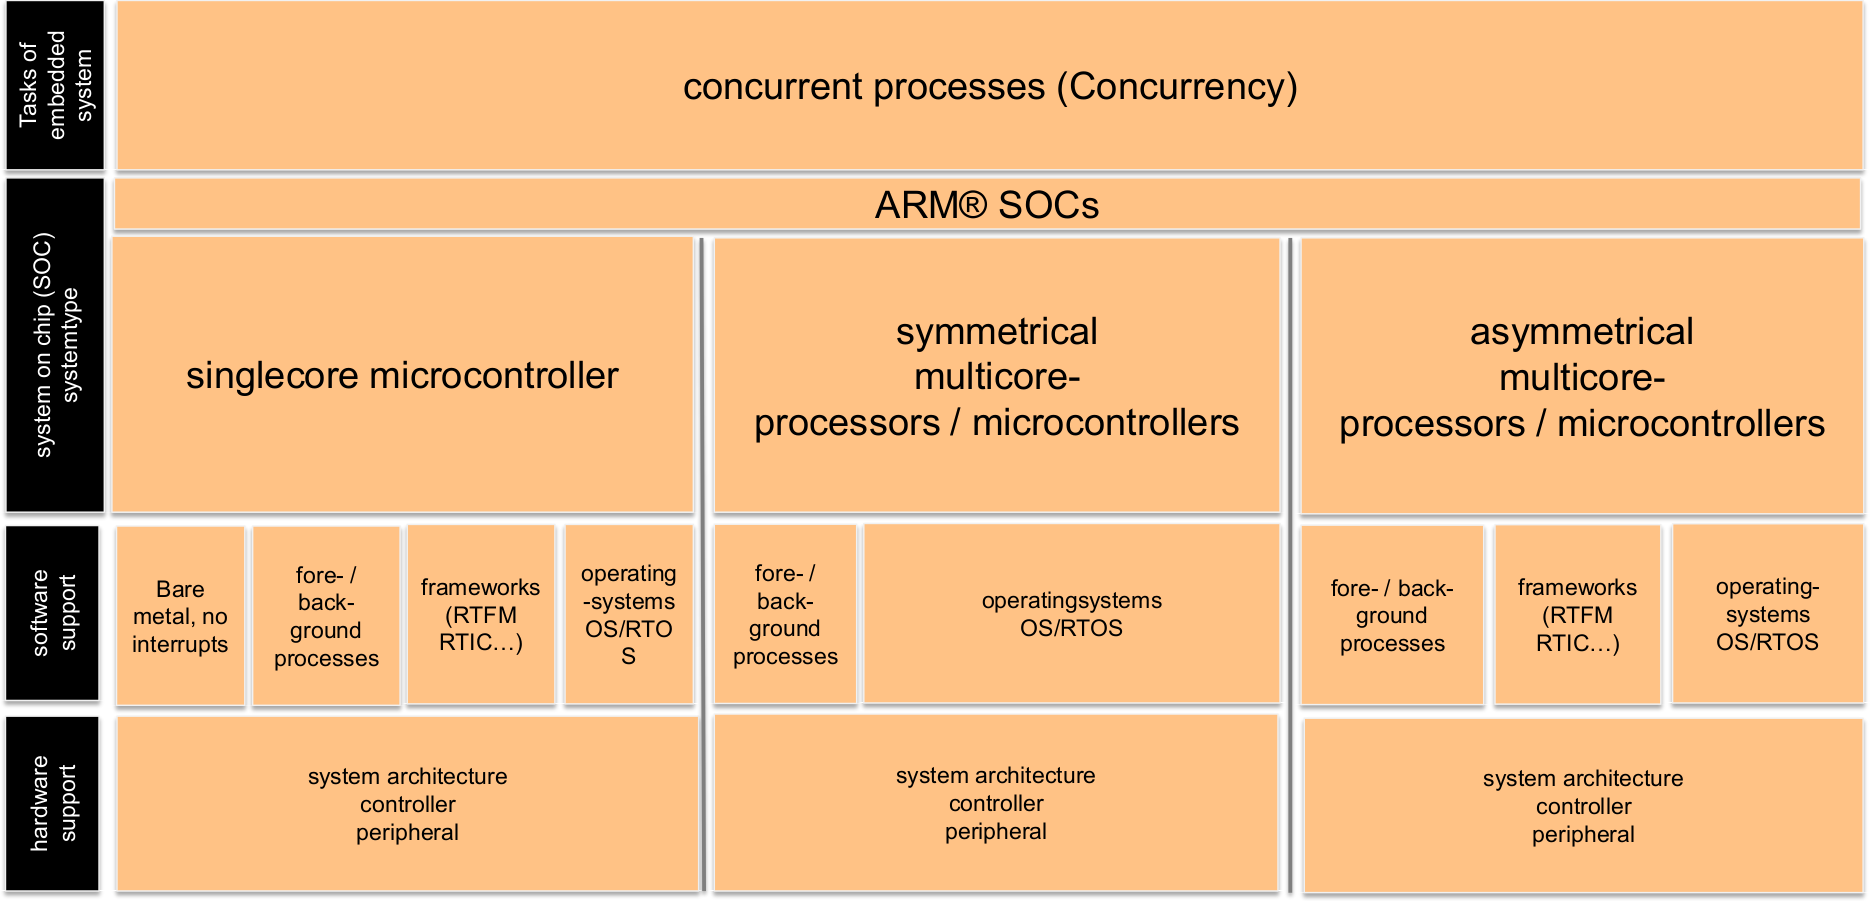
\includegraphics[width=\textwidth]{images/RTSystems/emb_landscape.png}

\subsection{Architectures}
\begin{tabularx}{\textwidth}{lXX}\hline
  Architecture & Von-Neumann                                                             & Harvard                                                             \\\hline
  Bus          & One bus for instructions and data                                       & Two seperate busses for instructions and data                       \\
  Pros         & + Cost effective design                                                 & + Better conditions for concurrency                                 \\
  Cons         & - Slower                                                                & - Costly                                                            \\
               & 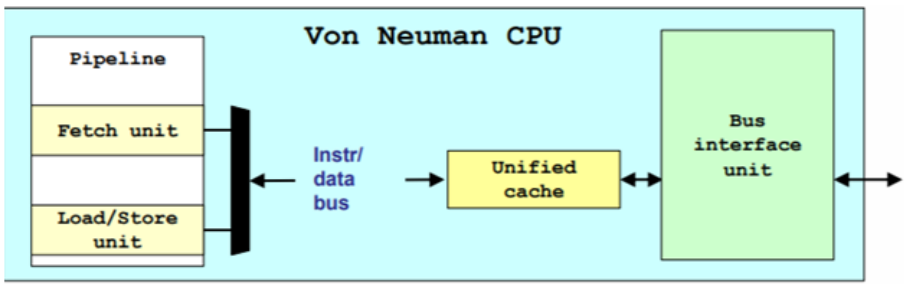
\includegraphics[width=0.4\textwidth]{images/RTSystems/von_neumann.png} & 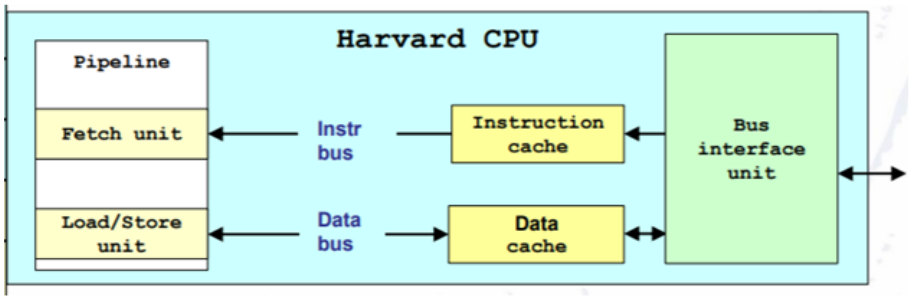
\includegraphics[width=0.4\textwidth]{images/RTSystems/harvard.png} \\\hline
\end{tabularx}

Real time support of hardware depends on:
\begin{itemize}
  \item Bus architecture
  \item CPU commands
  \item Interrput controller
\end{itemize}